\documentclass{article}
\usepackage[a4paper, margin=1in]{geometry}
\usepackage{amsmath}
\usepackage{graphicx}
\usepackage{hyperref}
\usepackage{amssymb}
\usepackage{makecell}

\title{Parallelized Exact k-Nearest Neighbors Implementation}
\author{Rousomanis Georgios (10703)\\
Department of Electrical and Computer Engineering\\
Aristotle University of Thessaloniki\\
Email: rousoman@ece.auth.gr
}

\begin{document}
\maketitle

\section{Introduction}

The goal of this project is to develop an efficient parallel solution to the 
\textbf{approximate all-to-all nearest neighbors (ANN)} problem. This task is crucial in 
large-scale data analysis applications, where computing exact all-to-all $k$-nearest neighbors 
becomes computationally infeasible due to the quadratic complexity in both runtime and memory. 

As a first step, we implemented a highly optimized and parallelized 
\textbf{exact k-Nearest Neighbors (k-NN)} algorithm to establish a baseline for correctness and 
to study the performance characteristics of parallel execution strategies. This implementation 
allowed us to gain valuable insights into memory management, batching strategies, and parallel 
workload distribution across multiple threading models.

Building on these foundations, we extended the approach to the more challenging 
\textbf{approximate all-to-all nearest neighbors} problem using a clustering-based approximation 
strategy. This method reduces the computational cost by partitioning the dataset into smaller 
subsets and performing local exact k-NN computations, allowing for significant acceleration
with a controlled trade-off in accuracy.

Our work systematically evaluates the accuracy, throughput, and scalability of the proposed 
methods under different parallelization frameworks (Pthreads, OpenMP, OpenCilk), cluster 
granularities, and thread configurations.

\section{k-Nearest Neighbors Implementation}

\subsection{Problem Definition}

The \textbf{k-Nearest Neighbors (k-NN)} problem involves finding, for each query point, the $k$ 
closest points from a reference corpus according to a specified distance metric. Formally, given 
a set of $N$ data points (the corpus) $C \in \mathbb{R}^{N \times D}$ and a set of $M$ query 
points $Q \in \mathbb{R}^{M \times D}$, the goal is to identify, for each $q_i \in Q$, the $k$ 
nearest neighbors in $C$ based on pairwise distances.

In this implementation, the \textbf{squared Euclidean distance} is used, which can be efficiently 
computed in matrix form without explicit loops. The pairwise distance matrix 
$D \in \mathbb{R}^{M \times N}$ between $Q$ and $C$ is calculated as:

\[
D = \|Q\|^2 + \|C\|^2 - 2 Q C^\top
\]

where:
\begin{itemize}
    \item $\|Q\|^2$ is the vector of squared norms of the query points, broadcasted across columns,
    \item $\|C\|^2$ is the vector of squared norms of the corpus points, broadcasted across rows,
    \item $Q C^\top$ is the matrix of dot products between query and corpus points.
\end{itemize}

This formulation avoids explicit nested loops and enables the use of optimized matrix multiplication 
routines for efficient distance computation.

\subsection{Algorithm Overview}

\subsubsection{Memory Management}
Efficient memory management is essential due to the $O(N^2)$ complexity of pairwise distance computations. 
The algorithm employs the following strategies:

\begin{itemize}
    \item \textbf{Batch Size Estimation:} The batch size $B$ is determined at runtime based on a user-defined 
    fraction of available system memory (e.g., 50\%), ensuring intermediate buffers (distance matrices, norms,
    results) remain within safe memory limits.
    
    \item \textbf{Batch Processing:} Queries are processed in batches of size $B$, reducing peak memory usage 
    from $O(N^2)$ to $O(B \times N)$ while enabling efficient blocked matrix operations.
    
    \item \textbf{Preallocation and Reuse:} Temporary buffers for norms, distances, and neighbor indices are 
    preallocated once and reused across batches, minimizing allocation overhead and avoiding heap fragmentation.
\end{itemize}

\subsubsection{Parallelization Strategy}

The main computational bottleneck of the algorithm lies in two stages: (i) the matrix multiplication between 
the query batches and the corpus, and (ii) the $k$-selection step to extract the nearest neighbors. To address
this, parallelism is applied across both stages as follows:

\begin{enumerate}
    \item \textbf{Workload Distribution:} Each batch of queries is partitioned into contiguous blocks of 
    memory, with each thread responsible for processing a disjoint subset of the queries. This approach ensures 
    cache-friendly memory access and minimizes false sharing.
    
    \item \textbf{Dot Product Computation:} Within each batch, each thread independently computes dot products
    between its assigned query vectors and the full corpus. Matrix multiplication is performed via OpenBLAS 
    in single-threaded mode to avoid thread contention with the outer parallel loop.
    
    \item \textbf{$k$-Selection Step:} After computing pairwise distances, each thread executes a partial 
    sorting procedure (using \texttt{QuickSelect}) on its assigned queries to efficiently determine the $k$ 
    nearest neighbors without fully sorting all distances.
    
    \item \textbf{Thread Synchronization:} Upon completing the computations for their assigned queries 
    within a batch, all threads synchronize implicitly at the batch boundary. The program then proceeds to 
    the next batch, maintaining strict batch-wise independence to prevent data hazards.
\end{enumerate}

\subsubsection{Parallelization Methods}

\paragraph{Pthreads Implementation}

\begin{itemize}
    \item A fixed-size thread pool is created explicitly at the start of the program and remains active 
    throughout execution, eliminating the overhead of repeated thread creation and destruction.
    \item Synchronization is handled manually using mutexes and condition variables to coordinate thread activity.
    \item Upon program completion, the thread pool along with all auxiliary data structures are properly destroyed 
    to ensure clean resource deallocation.
\end{itemize}

\paragraph{OpenMP Implementation}

\begin{itemize}
    \item Thread management is fully automated: threads are spawned and managed by the OpenMP runtime, 
    with no need for manual thread pool creation.
    \item Synchronization and workload distribution are handled implicitly via compiler directives, such as 
    \texttt{\#pragma omp parallel for}, reducing developer effort and minimizing synchronization code.
    \item Upon completion of parallel regions, OpenMP automatically manages thread teardown and resource 
    cleanup, requiring no manual intervention for deallocation.
\end{itemize}


\paragraph{OpenCilk Implementation}

\begin{itemize}
    \item The OpenCilk runtime handles task parallelism dynamically through a work-stealing scheduler, 
    eliminating the need for manual thread management or explicit thread pools.
    \item Synchronization is implicit, with the runtime ensuring correct execution order via the fork-join 
    model, removing the need for explicit locks or condition variables.
    \item Task and resource cleanup are fully managed by the OpenCilk runtime, allowing developers to focus 
    solely on expressing parallelism via \texttt{cilk\_for} without manual resource deallocation.
\end{itemize}

\begin{table}[h]
\centering
\begin{tabular}{|l|c|c|c|}
\hline
\textbf{Aspect} & \textbf{Pthreads} & \textbf{OpenMP} & \textbf{OpenCilk} \\
\hline
Thread Management & \makecell{Manual \\ fixed thread pool} & \makecell{Automatic \\ runtime threads} & \makecell{Dynamic tasks \\ with work-stealing} \\
\hline
Synchronization & \makecell{Manual \\ (mutexes, cond vars)} & \makecell{Implicit \\ via pragmas} & \makecell{Implicit \\ via fork-join} \\
\hline
Resource Cleanup & \makecell{Manual \\ destruction} & \makecell{Automatic \\ cleanup} & \makecell{Automatic \\ cleanup} \\
\hline
\end{tabular}
\caption{Comparison of Pthreads, OpenMP, and OpenCilk implementations}
\end{table}

\subsection{Validation of the Algorithm}

The validation process ensures the correctness of the implemented k-nearest neighbors algorithm by 
systematically comparing its output against a reliable reference.

\begin{enumerate}
    \item \textbf{Test Data Generation:} A diverse set of test cases is generated, including both fixed and
    randomized datasets. For each test case, the ground truth nearest neighbors and distances are computed 
    using a trusted, well-established k-NN implementation. These reference results serve as the standard for
    correctness.
    
    \item \textbf{Algorithm Execution:} The algorithm under test processes each generated query set against 
    the corresponding corpus, producing estimated nearest neighbors and distance values.
    
    \item \textbf{Result Comparison:} The output distances and neighbor indices from the tested algorithm 
    are compared element-wise against the reference results within a specified numerical tolerance. Both 
    the distances and indices must match to validate correctness.
    
    \item \textbf{Reporting:} Each test case outcome is reported individually as pass or fail. The overall 
    success of the validation is determined by aggregating these results, ensuring comprehensive verification 
    across varying dataset sizes and dimensions.
\end{enumerate}

This procedure rigorously validates the implementation by leveraging precomputed reference results and 
enforcing strict numerical and index consistency checks.

\subsection{Performance of the Algorithm}

\subsubsection{Benchmarking Procedure}

The benchmarking procedure assesses the performance scalability of the k-nearest neighbors implementation 
using the \textbf{MNIST} dataset. The experiments are designed to evaluate how execution time and throughput 
vary with different parallelization methods and thread counts.

\begin{enumerate}
    \item The corpus and query matrices are loaded from the MNIST dataset.
    \item The algorithm executes the k-NN search for six thread configurations: 
    1, 2, 4, 8, 16, and 32 threads.
    \item Each configuration is evaluated under three parallelization models: Pthreads, OpenMP, and OpenCilk.
    \item For every run, the execution time is measured, and throughput is calculated in queries processed 
    per second.
    \item All experiments were conducted on a system running Ubuntu LTS 22.04 with a 4-core processor, 
    allowing evaluation of performance scaling both within and beyond the physical core count.
\end{enumerate}

This procedure enables direct comparison of parallelization strategies in terms of efficiency and scalability
across varying thread counts.

\subsubsection{Benchmark Results}

The benchmark results are summarized in Figure~\ref{fig:knn_throughput_vs_threads}, which presents the 
throughput (queries processed per second) of the k-NN implementation as a function of the number of 
threads used by the application. Separate plots are provided for each of the three parallelization methods: 
Pthreads, OpenMP, and OpenCilk.

For each method, two curves are depicted:
\begin{itemize}
\item A \textbf{solid line} shows the throughput when the application itself is parallelized across multiple
threads while OpenBLAS is restricted to a single thread. This represents the scenario where all parallel 
resources are allocated to the k-NN search procedure.
\item A \textbf{dashed horizontal line} indicates the throughput when the application runs on a single thread 
while OpenBLAS utilizes all available system cores. This serves as a baseline for the performance attainable 
through multi-threaded BLAS operations alone, without application-level parallelization.
\end{itemize}

Across all three parallelization strategies, the solid lines exhibit similar behavior. As the number of 
application threads increases, the throughput rises, reaching a peak when the thread count matches the 
number of physical CPU cores (four in our test system). Beyond this point, the throughput begins to decline. 
This drop is attributed to the overhead introduced by excessive threading, such as increased context-switching,
resource contention, and scheduling inefficiencies on the limited number of cores.

Importantly, the peak throughput achieved using the application’s own parallelization (solid line) consistently
surpasses the performance achieved by relying solely on OpenBLAS parallelism (dashed line). This demonstrates the
effectiveness of explicit workload distribution at the application level, allowing better utilization of compute 
resources for the specific access patterns and memory requirements of the k-NN search.

Overall, the results highlight both the scalability limits imposed by hardware constraints and the advantages 
of integrating parallelism directly into the k-NN algorithm, beyond relying solely on low-level numerical 
libraries.

\begin{figure}
    \centering
    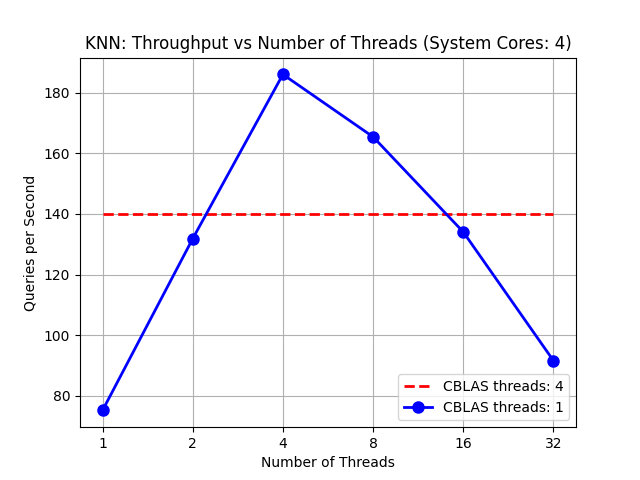
\includegraphics[width=0.5\linewidth]{figures/knn_throughput_vs_threads.png}
    \caption{Throughput of the exact k-Nearest Neighbors algorithm as a function of the number of threads used. 
    Solid lines show application-level parallelization with OpenBLAS restricted to a single thread, while dashed
    lines represent single-threaded application execution with multi-threaded OpenBLAS.}
    \label{fig:knn_throughput_vs_threads}
\end{figure}


\section{Approximate All-to-All Nearest Neighbors Implementation}

\subsection{Problem Definition}

The \textbf{approximate all-to-all nearest neighbors (ANN)} problem involves computing, for each data 
point in a corpus $C \in \mathbb{R}^{N \times D}$, its $k$ nearest neighbors among all other points 
in $C$. This differs from traditional k-NN queries in that the queries and the corpus are identical,
and the goal is to approximate the nearest neighbors efficiently. 

Due to the $O(N^2)$ computational and memory complexity of exact all-to-all k-NN search, the objective 
is to develop an approximate solution that reduces runtime and memory footprint, while maintaining 
acceptable recall accuracy. 

In this implementation, we adopt a clustering-based approach to divide the corpus into smaller subsets 
(clusters), solve exact k-NN within each cluster, and optimize workload distribution through multi-threading.

\subsection{Algorithm Overview}

The algorithm follows a two-stage pipeline:
\begin{itemize}
    \item \textbf{Stage 1: Clustering.} The data points are partitioned into clusters using a lightweight
    k-means variant. To ensure cluster quality, small clusters are merged until all clusters contain more 
    than $k$ points, enabling valid intra-cluster k-NN computation.
    \item \textbf{Stage 2: Intra-cluster k-NN.} For each cluster, exact k-NN search is performed internally.
    Since points are only compared within their assigned clusters, the approach approximates the full $k$-NN 
    graph.
\end{itemize}

This pipeline reduces the overall number of distance computations while leveraging parallelization for 
intra-cluster k-NN computations.

\subsubsection{Clustering Strategy}

The clustering stage uses a randomized initialization followed by a single assignment step:
\begin{itemize}
    \item \textbf{Initialization:} A fixed number of $K_c$ points are randomly selected from the corpus 
    to serve as initial centroids. The remaining points are assigned to the nearest centroid using exact 
    distance computations.
    \item \textbf{Merging Strategy:} After the initial assignment, clusters with fewer than $k$ points 
    are identified and iteratively merged into their nearest neighboring valid cluster based on centroid 
    distances. This ensures that each cluster has enough points to perform $k$-NN search locally.
    \item \textbf{Centroid Update:} Following merging, centroids are recomputed by averaging the points 
    within each cluster.
\end{itemize}

This clustering procedure is executed once prior to k-NN computation, providing a balanced cluster 
distribution and preventing invalid or degenerate clusters.

\subsubsection{Workload Distribution}

After clustering, intra-cluster k-NN searches are distributed across threads using a 
\textbf{greedy bin-packing algorithm} based on cluster sizes:
\begin{itemize}
    \item \textbf{Cluster Assignment:} Clusters are sorted by size in descending order. Each cluster is 
    assigned to the thread with the smallest cumulative workload (sum of points across its assigned clusters).
    \item \textbf{Thread Tasks:} Each thread processes its assigned clusters independently, performing exact 
    $k$-NN within each cluster.
    \item \textbf{Memory Optimization:} Threads dynamically adjust their memory usage based on the number of 
    points they process relative to the total number of points, ensuring adherence to a global maximum memory 
    usage ratio.
\end{itemize}

This strategy minimizes load imbalance by ensuring that larger clusters are evenly distributed across threads,
improving parallel efficiency.

\subsubsection{Parallelization Strategy (pros \& cons)}

The approximate ANN algorithm simplifies parallelization by assigning each thread a fixed subset of clusters 
only once before computation starts. This static workload distribution offers advantages but also introduces 
challenges related to load balancing.

\begin{itemize}
    \item Static assignment avoids repeated thread pool creation and dynamic batching, making the Pthreads 
    implementation simpler—threads are created once, process their assigned clusters independently, then 
    joined at the end.
    \item However, cluster size variability can cause load imbalance, as some threads may handle more data than 
    others; this contrasts with exact k-NN’s dynamic batching which enables more balanced workload distribution.
    \item To address imbalance, heuristics like greedy bin-packing are used for cluster assignment, while OpenMP's
    static scheduling and OpenCilk’s dynamic work-stealing help redistribute work at runtime.
    \item Overall, this approach reduces thread management overhead but requires careful workload distribution 
    to maintain parallel efficiency.
\end{itemize}

\subsection{ANN Benchmarks}

\subsubsection{Benchmarking Procedure}

This benchmark assesses the trade-off between accuracy and execution time of the approximate all-to-all 
nearest neighbors (ANN) algorithm under different configurations, including the number of clusters, 
thread counts, and parallelization methods. The key steps are:

\begin{itemize}
    \item Loading and concatenating the training and test subsets of the MNIST dataset.
    \item Computing the exact all-to-all nearest neighbors on the combined dataset using Euclidean distance 
    as a metric of proximity.
    \item Executing the ANN algorithm with various cluster counts and parallelization modes, recording 
    throughput and recall by comparison to the exact results.
\end{itemize}

\subsubsection{Recall vs Throughput}

The approximate all-to-all nearest neighbors algorithm involves a fundamental tradeoff between accuracy 
(recall) and computational efficiency (throughput). This tradeoff is primarily governed by the number of 
clusters used to partition the dataset: fewer clusters yield coarser partitions that tend to retain more 
true neighbors within the same cluster, improving recall but increasing computation time; conversely, 
more clusters create finer partitions that reduce workload and increase throughput at the cost of 
potentially missing some true neighbors.

Figure~\ref{fig:ann_recall_vs_clusters} illustrates how recall degrades as the number of clusters increases, 
with high accuracy (up to 90\%) achieved at low cluster counts (around 5) and recall dropping below 60\% as 
clusters approach 100. This confirms the expected impact of cluster granularity on approximation quality.

The combined effect of this tradeoff on performance is presented in Figure~\ref{fig:ann_recall_vs_throughput},
which plots recall against throughput for three parallelization methods—Pthreads, OpenMP, and OpenCilk—across 
multiple cluster counts ($K_c = 5, 10, 20, 50, 100$). All implementations yield consistent recall values for 
each cluster count and demonstrate comparable throughput, highlighting the stability of the algorithm across 
parallel frameworks. This visualization enables users to select an appropriate cluster count to balance speed 
and accuracy according to their application requirements.

\subsubsection{Throughput Scaling with Number of Threads}

Figure~\ref{fig:ann_throughput_vs_threads} illustrates throughput scaling with respect to the number of 
threads for different cluster counts $K_c$. Across all cases, throughput increases with thread count, 
peaking around the number of physical CPU cores.

For smaller $K_c$ (e.g., 5, 10, 20), throughput flattens beyond the core count. This occurs because 
the limited number of large clusters results in significant workload imbalance—execution time is 
dominated by the largest cluster, leaving extra threads underutilized.

In contrast, for higher $K_c$ (e.g., 50, 100), throughput exhibits a clearer ``elbow'' behavior: it 
increases up to the physical core count and then drops slightly. The larger number of clusters improves 
workload distribution across threads, but the overhead of thread oversubscription (e.g., context switching) 
prevents further scaling.

Similar trends are observed for OpenMP and OpenCilk, with OpenCilk often providing smoother scaling due to 
dynamic work stealing.

\begin{figure}
    \centering
    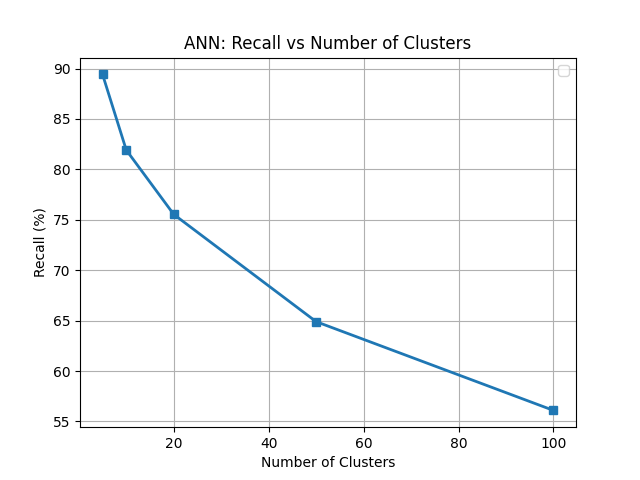
\includegraphics[width=0.5\linewidth]{figures/ann_recall_vs_clusters.png}
    \caption{Recall of the approximate all-to-all nearest neighbors algorithm as a function of the number of clusters}
    \label{fig:ann_recall_vs_clusters}
\end{figure}

\begin{figure}
    \centering
    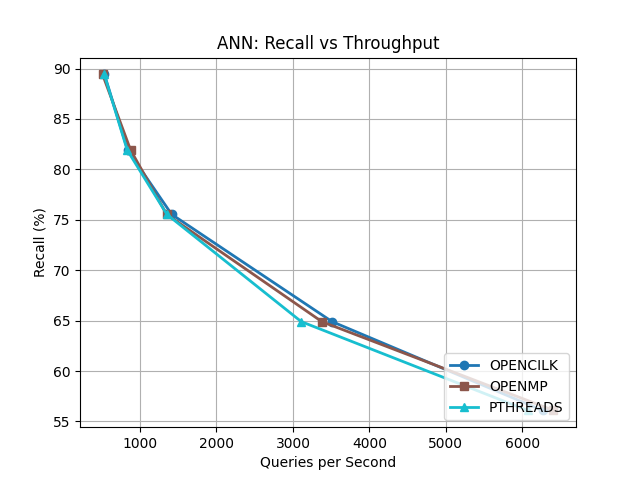
\includegraphics[width=0.5\linewidth]{figures/ann_recall_vs_throughput.png}
    \caption{Recall versus throughput for the approximate all-to-all nearest neighbors algorithm using 
    Pthreads, OpenMP, and OpenCilk parallelization methods. Points correspond to cluster counts 
    $K_c = 5, 10, 20, 50,$ and $100$. }
    \label{fig:ann_recall_vs_throughput}
\end{figure}

\begin{figure}
    \centering
    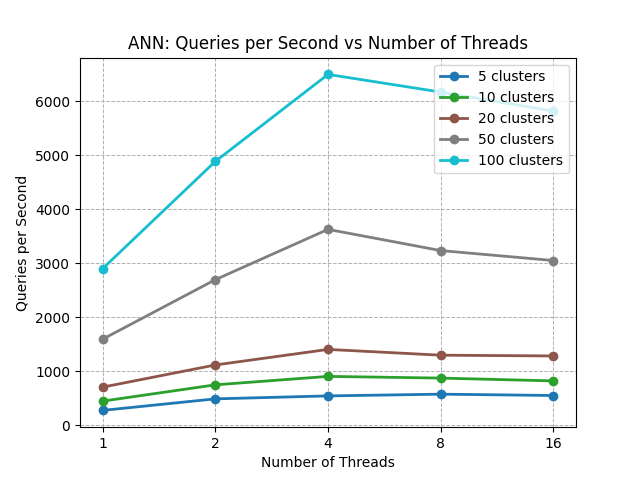
\includegraphics[width=0.5\linewidth]{figures/ann_throughput_vs_threads.png}
    \caption{Throughput vs number of threads for different cluster counts using Pthreads. Throughput 
    increases up to the physical core count and remains stable beyond. Higher cluster counts yield better 
    scaling due to improved workload balance.}
    \label{fig:ann_throughput_vs_threads}
\end{figure}

\section{Conclusion and Future Work}

In this project, we developed and evaluated parallel algorithms for both exact k-Nearest Neighbors (k-NN) 
and approximate all-to-all nearest neighbors (ANN) search. Starting with the exact k-NN implementation, 
we established a high-performance baseline, analyzing its scalability and performance under different 
parallelization strategies. Building upon this, we introduced a clustering-based approximation scheme 
for the ANN problem, significantly reducing computational costs while offering tunable trade-offs 
between accuracy and throughput.

Our benchmarking results demonstrated that:
\begin{itemize}
    \item The exact k-NN algorithm achieves good scalability up to the number of physical cores, with 
    explicit parallelization outperforming library-only threading.
    \item The ANN algorithm offers substantial speedups with controllable recall, where increasing the 
    number of clusters improves throughput at the cost of reduced accuracy.
    \item Multithreading achieves near-linear speedup up to core count, with OpenCilk providing smoother 
    scaling in scenarios with greater workload imbalance.
\end{itemize}

\textbf{Future work} will focus on further improving the quality and efficiency of the ANN solution. 
Key directions include:
\begin{itemize}
    \item \textbf{Merging neighbor lists across clusters} to reduce boundary effects and recover part 
    of the lost accuracy.
    \item \textbf{Exploring advanced clustering techniques}, such as balanced k-means or hierarchical 
    clustering, to achieve more uniform cluster sizes and minimize load imbalance.
    \item \textbf{Investigating hybrid parallelism} (e.g., combining OpenMP with SIMD vectorization) 
    to push performance beyond current thread-level parallelism.
    \item \textbf{Optimizing memory access patterns} for NUMA systems or GPUs to further accelerate 
    computation on modern hardware platforms.
\end{itemize}

Overall, our work highlights the practicality of clustering-based ANN methods in large-scale nearest 
neighbor computations and provides a flexible, parallelizable foundation for further extensions.


\end{document}
